\documentclass[
% -- opções da classe memoir --
article,			% indica que é um artigo acadêmico
12pt,				% tamanho da fonte
oneside,			% para impressão apenas no recto. Oposto a twoside
a4paper,			% tamanho do papel. 
% -- opções do pacote babel --
english,			% idioma adicional para hifenização
brazil,				% o último idioma é o principal do documento
sumario=tradicional
]{abntex2}
% ------------------------------
% Pacotes
% ------------------------------
\usepackage{lmodern}			% Usa a fonte Latin Modern
\usepackage[T1]{fontenc}	% Selecao de codigos de fonte.
% ------------------------------
% Posição da numeração da página
% ------------------------------
\usepackage{fancyhdr}
\pagestyle{fancyplain}
\fancyhf{}
\fancyhead[R]{\thepage}
%\renewcommand\headrulewidth{0pt}% default ist .4pt
\renewcommand{\plainheadrulewidth}{0pt}
% ------------------------------
% Equações
\usepackage{mathtools}
\usepackage{amsmath}
\usepackage{chemformula}
% ------------------------------
% Seleção de tamanho da fonte das seções
\usepackage{titlesec}
\titleformat*{\section}{\normalsize \bfseries\sffamily} %Seleciona o tamanho da fonte da section 
\titleformat*{\subsection}{\normalsize \bfseries\sffamily} %Seleciona o tamanho da fonte da subsection
\titleformat*{\subsubsection}{\normalsize \sffamily} %Seleciona o tamanho da fonte da subsubsection
% ------------------------------
\usepackage[utf8]{inputenc}		% Codificacao do documento (conversão automática dos acentos)
\usepackage{indentfirst}		% Indenta o primeiro parágrafo de cada seção.
\usepackage{nomencl} 			% Lista de simbolos
\usepackage{color}				% Controle das cores
\usepackage{graphicx}			% Inclusão de gráficos
\usepackage{multirow}           % Usado para tabelas
\usepackage{microtype} 			% para melhorias de justificação
\usepackage{ragged2e}
\usepackage[top=3cm, bottom=2cm, left=3cm, right=2cm]{geometry}
% ------------------------------
% Pacotes adicionais, usados apenas no âmbito do Modelo Canônico do abnteX2
% ---
\usepackage{lipsum}				% para geração de dummy text
% ------------------------------
% Pacotes de citações
\usepackage[brazilian,hyperpageref]{backref}	 % Paginas com as citações na bibl
\usepackage[alf]{abntex2cite}	% Citações padrão ABNT
% ------------------------------
% Informações de dados para CAPA e FOLHA DE ROSTO ---
\titulo{ \textsf{\textbf{MODELO DE ARTIGO CIENTÍFICO COM \abnTeX - UERN}}}
\tituloestrangeiro{}

\autor{
	Equipe \abnTeX \thanks{Responsável pela elaboração do modelo canônico no qual este trabalho se baseia. \url{http://www.abntex.net.br/}} 
	\\[0.2cm] 
	Ruan Matheus\thanks{Aluno do curso de licenciatura em matemática pela UERN. } }
\local{Brasil}
\data{2023}
% ------------------------------
% Configurações de aparência do PDF final
% ------------------------------
% alterando o aspecto da cor azul
\definecolor{blue}{RGB}{41,5,195}

% informações do PDF
\makeatletter
\hypersetup{
	%pagebackref=true,
	pdftitle={\@title}, 
	pdfauthor={\@author},
	pdfsubject={Modelo de artigo científico com abnTeX2},
	pdfcreator={LaTeX with abnTeX2},
	pdfkeywords={abnt}{latex}{abntex}{abntex2}{atigo científico}, 
	colorlinks=true,       		% false: boxed links; true: colored links
	linkcolor=blue,          	% color of internal links
	citecolor=blue,        		% color of links to bibliography
	filecolor=magenta,      		% color of file links
	urlcolor=blue,
	bookmarksdepth=4
}
% ------------------------------
\makeatother
% compila o indice
\makeindex
% ------------------------------
% Espaçamentos entre linhas e parágrafos 
% ------------------------------
% O tamanho do parágrafo é dado por:
\setlength{\parindent}{1.25cm}
% ------------------------------
% Controle do espaçamento entre um parágrafo e outro:
\setlength{\parskip}{0.2cm}  % tente também \onelineskip
% ------------------------------
% Espaçamento simples
\SingleSpacing
% ------------------------------
\makeatletter
\let\@fnsymbol\@arabic
\makeatother		
% ------------------------------
% Ajuste das informações da capa
\makeatletter
\def\@maketitle{
	\newpage
	\null
	\vskip 2em
	\begin{center}
		\let \footnote \thanks
		{\normalsize \@title \par}
		\vskip 3em
		{\normalsize \flushright
			\lineskip .5em
			\begin{tabular}[t]{c}
				\@author
			\end{tabular}\par}
		\vskip 1em
		%{\large \@date}%
	\end{center}%
	\par
	\vskip 1.5em}
\makeatother
% ------------------------------
% Início do documento
% ------------------------------
\begin{document}
	
	% Seleciona o idioma do documento (conforme pacotes do babel)
	%\selectlanguage{english}
	\selectlanguage{brazil}
	
	% Retira espaço extra obsoleto entre as frases.
	\frenchspacing 
	
% -------------------------------
	% ELEMENTOS PRÉ-TEXTUAIS
% ------------------------------
	% Se desejar escrever o artigo em duas colunas, descomente a linha abaixo
	% e a linha com o texto ``FIM DE ARTIGO EM DUAS COLUNAS''.
	% \twocolumn[    		% INICIO DE ARTIGO EM DUAS COLUNAS
	%
	%---
% ------------------------------
	% página de titulo principal (obrigatório)
	\maketitle
	
	% resumo em português
	\begin{resumoumacoluna}[\normalsize \textsf{\textbf{RESUMO}}]
		Conforme as diretrizes do \emph{Manual de normalização de trabalhos acadêmicos da UERN}, disponível neste \href{https://www.uern.br/controledepaginas/manualtcc/arquivos/6762manual_de_tcc_uern_2022_finalizado.pdf}{link}, o resumo/abstract deve conter entre 100 e 250 palavras. O espaçamento entre linhas deve ser simples, com um único parágrafo recuado e texto justificado. A inclusão do resumo em língua estrangeira é facultativa, conforme a ABNT NBR 6022:2018. As palavras-chave devem ser precedidas por dois pontos, separadas por ponto e vírgula, e finalizadas por ponto. Devem ser escritas com letras minúsculas, com exceção de substantivos próprios e nomes científicos, sendo permitido o uso de no máximo 5 palavras-chave.
		
		\vspace{\onelineskip}
		
		\noindent
		\textbf{Palavras-chave}: latex. abntex. UERN.
	\end{resumoumacoluna}
	% ------------------------------
	
	% resumo em inglês
	\renewcommand{\resumoname}{Abstract}
	\begin{resumoumacoluna}[\normalsize \textsf{\textbf{ABSTRACT}}]
		\begin{otherlanguage*}{english}
			In accordance with the guidelines of the UERN Academic Work Standardization Manual, available at this \href{https://www.uern.br/controledepaginas/manualtcc/arquivos/6762manual_de_tcc_uern_2022_finalizado.pdf}{link}, the abstract should contain between 100 and 250 words. Line spacing should be single, with a single indented paragraph and justified text. The inclusion of an abstract in a foreign language is optional, in accordance with ABNT NBR 6022:2018. Keywords should be preceded by a colon, separated by semicolons, and ended with a period. They should be written in lowercase letters, except for proper nouns and scientific names, and a maximum of 5 keywords are allowed.
			
			\vspace{\onelineskip}
			
			\noindent
			\textbf{Keywords}: latex. abntex. UERN.
		\end{otherlanguage*}  
	\end{resumoumacoluna}
% ------------------------------
% ------------------------------
% A data de submissão do artigo é um elemento obrigatório, porém é relevante apenas para publicação de artigos em revistas/anuais. Caso queira exibir a data de submissão do artigo, descomente as linhas a seguir:
	
	%\begin{center}\smaller
		%\textbf{Data de submissão e aprovação}: %elemento obrigatório. Indicar dia, mês e ano
		
		%\textbf{Identificação e disponibilidade}: %elemento opcional. Pode ser indicado 
		%o endereço eletrônico, DOI, suportes e %outras informações relativas ao acesso.
	%\end{center}
	
	% ------------------------------
	% ELEMENTOS TEXTUAIS
	% ------------------------------
	\textual
	% ------------------------------
	% Introdução
	% ------------------------------
	\section{INTRODUÇÃO}
	
	Além das normas comuns da ABNT, é habitual que as instituições de ensino possuam suas próprias regulamentações para a padronização de trabalhos acadêmicos. No caso da UERN, há um manual que estabelece as diretrizes de padronização para os trabalhos acadêmicos produzidos pela instituição. O manual pode ser acessado através do link a seguir: \url{https://www.uern.br/controledepaginas/manualtcc/arquivos/6762manual_de_tcc_uern_2022_finalizado.pdf}
	
	Este trabalho é um exemplo de artigo científico elaborado utilizando o \LaTeX, com a classe \abnTeX, seguindo as orientações do manual de trabalhos acadêmicos da UERN. O objetivo é simplificar a produção de artigos técnicos/científicos utilizando o \LaTeX $~$ e que estejam em conformidade com as normas específicas da UERN.
	
	Este arquivo está disponível de forma gratuita para livre uso, modificação e distribuição, conforme os termos da “\emph{The \LaTeX $~$ Project Public License}\footnote{\url{https://www.latex-project.org/lppl.txt}}”. Não sou o autor do arquivo usado como referência, apenas ajustei o modelo padrão fornecido pela equipe \abnTeX $~$ e \emph{Lauro César Araujo}. Os links para o projeto da equipe \abnTeX $~$ estarão disponíveis no final deste trabalho.
    % ------------------------------
	% Seção de explicações
    % ------------------------------
	\section{PERSONALIZAÇÕES}

    No que diz respeito a artigos técnicos/científicos, o manual de trabalhos acadêmicos da UERN apresenta poucas alterações específicas, se comparado com as normas gerais da ABNT. Se você deseja apenas redigir um artigo técnico/científico que esteja em conformidade com as normas da UERN, não é recomendável fazer modificações na formatação deste documento. No entanto, se necessário, é possível personalizar todas as seções deste documento de acordo com suas necessidades.

    Por conveniência, serão destacadas apenas as formas de alterar as principais características do trabalho, como o tamanho da fonte, as margens, o espaçamento e as informações da capa. Para obter mais opções de formatação, consulte a documentação fornecida pela equipe \abnTeX, disponível através deste link: \url{https://linorg.usp.br/CTAN/macros/latex/contrib/abntex2/doc/abntex2.pdf}.
 
	\subsection{Tamanho da fonte}

    A fonte a ser utilizada no documento, incluindo o título do artigo, títulos de seções e subseções, deve ser tamanho 12. Além disso, o manual de trabalhos acadêmicos define as seguintes normas para numeração sucessiva das seções do trabalho:
    
    % ------------------------------
    % Início da tabela
    % ------------------------------
    \begin{table}[ht!]
    \begin{tabular}{ |p{5cm}||p{4cm}||p{3cm}||p{3cm}|  }
 \hline
 \multicolumn{4}{|c|}{Numeração sucessiva das seções} \\
 \hline
 Tipo de seção & Código \LaTeX & Fonte & Negrito\\
 \hline
 \textbf{1 SEÇÃO PRIMÁRIA}   & \verb|\section| & MAIÚSCULA &   \textbf{Sim} \\
 \textbf{1.1 Seção secundária} &  \verb|\subsection| & Minúscula   & \textbf{Sim} \\
 1.1.1 Seção terciária & \verb|\subsubsection| & Minúscula &  Não \\
 1.1.1.1 Seção quaternária & \verb|\subsubsubsection| & Minúscula &  Não\\
 \hline
\end{tabular}
\caption{Numeração sucessiva das seções. Fonte: Manual de trabalhos acadêmicos da UERN.}
\label{Tabela 1}
\end{table}
	% ------------------------------
    % Fim da tabela
    % ------------------------------


    No \LaTeX, o tamanho da fonte é geralmente definido por meio de códigos. A tabela a seguir apresenta os principais códigos para modificar o tamanho da fonte, além do seu tamanho aproximado em comparação com outros editores, como o \texttt{Microsoft Word} ou \texttt{Libre Office}.

    % ------------------------------
    % Início da tabela
    % ------------------------------
    \begin{table}[h!]
    \begin{tabular}{ |p{5cm}||p{4cm}|}
 \hline
 \multicolumn{2}{|c|}{Tamanho da fonte para um documento em 12pt} \\
 \hline
 Comando & Tamanho em pt \\
 \hline
 \verb|\tiny | & \texttt{6pt} \\
 \verb|\scriptsize | & \texttt{8pt} \\
 \verb|\footnotesize | & \texttt{10pt} \\
 \verb|\small | & \texttt{10.95pt}  \\ \verb|\normalsize | & \texttt{12pt} \\ \verb|\large | & \texttt{14.4pt} \\ \verb|\Large| & \texttt{17.28} \\ \verb|\LARGE | & \texttt{20.74} \\ \verb|\huge| & \texttt{24.88}\\
 \hline
\end{tabular}
\caption{Comparação de tamanho da fonte.}
\label{Tabela 2}
\end{table}
	% ------------------------------
    % Fim da tabela
    % ------------------------------

    \subsubsection{Alteração do tamanho da fonte em todo o documento}
  
   O tamanho padrão das letras é definido no preâmbulo\footnote{No uso do \LaTeX, entende-se como "preâmbulo" toda a informação que vem no início do documento, antes do código begin\{document\}.} do código pela linha a seguir.

    \begin{verbatim}
        \documentclass[article, 12pt]{abntex2}
    \end{verbatim}

    Para alterar o tamanho da fonte em \textbf{TODO} o documento, altere a opção \texttt{"12pt"} para o tamanho desejado.
    
    \subsubsection{Alteração do tamanho da fonte do título do trabalho}

    Para alterar o tamanho da fonte do título do trabalho, procure a seção \texttt{"Ajuste das informações da capa"} no preâmbulo deste arquivo e altere o código \verb|\normalsize| da seguinte linha:

    \begin{verbatim}
        {\normalsize \@title \par}
    \end{verbatim}

    \subsubsection{Alteração do tamanho da fonte nas seções do trabalho}

    Procure a seção \texttt{"Seleção de tamanho da fonte das seções"} no preâmbulo e altere o comando \verb|\normalsize| das seguintes linhas, conforme necessário:

    \begin{verbatim}
    \titleformat*{\section}{\normalsize \bfseries\sffamily} 
    \titleformat*{\subsection}{\normalsize \bfseries\sffamily}
    \titleformat*{\subsubsection}{\normalsize \sffamily} 
    \end{verbatim}

    \subsection{Margens e espaçamento}

    As margens do lado esquerdo, direito, superior e inferior deste arquivo estão de acordo com o Manual de Trabalhos Acadêmicos, sendo, respectivamente, 3 cm, 2 cm, 3 cm e 2 cm. Não é necessário modificar as margens do documento, mas se desejar, você pode alterar os valores numéricos na linha de código a seguir no início do documento:

    \begin{verbatim}
    \usepackage[top=3cm, bottom=2cm, left=3cm, right=2cm]{geometry}
    \end{verbatim}

    O arquivo já possui espaçamento simples entre linhas definido. O recuo do parágrafo e o espaço entre parágrafos são configurados, respectivamente, pelos valores numéricos das seguintes linhas de código no início do documento:

    \begin{verbatim}
    \setlength{\parindent}{1.25cm}
    \setlength{\parskip}{0.2cm}
    \end{verbatim}

    \subsection{Informações da capa}

    O Manual de Trabalhos Acadêmicos da UERN estabelece que a capa de artigos técnicos/científicos deve conter apenas o título do trabalho e os nomes dos autores. No entanto, em algumas situações, é possível que o autor opte por incluir também informações como o nome da instituição, a faculdade, o curso e/ou o nome da disciplina.

    Para realizar a inclusão dessas informações, siga os passos a seguir:

    \begin{enumerate}
       \item Criar os comandos \texttt{"Instituicao"}, \texttt{"faculdade"}, \texttt{"curso"} e \texttt{"disciplina"}. 
       
       Para isso, adicione as seguintes linhas de código no preâmbulo do arquivo. Lembre de substituir as informações pertinentes conforme sua necessidade:

    \begin{verbatim}
\newcommand{\inst}{UNIVERSIDADE DO ESTADO DO RIO GRANDE DO NORTE - UERN}
\newcommand{\fac}{FACULDADE DE CIÊNCIAS EXATAS E NATURAIS - FANAT}
\newcommand{\curso}{LICENCIATURA EM MATEMÁTICA}
\newcommand{\disc}{USO DO LATEX}
\end{verbatim}

       
        \item Localizar a seção \texttt{"Ajuste das informações da capa"} no preâmbulo do arquivo.

        \begin{verbatim}
\makeatletter
\def\@maketitle{
	\newpage
	\null
	\vskip 2em
	\begin{center}
		\let \footnote \thanks
		{\normalsize \@title \par}
		\vskip 3em
		{\normalsize \flushright
			\lineskip .5em
			\begin{tabular}[t]{c}
				\@author
			\end{tabular}\par}
		\vskip 1em
		%{\large \@date}%
	\end{center}%
	\par
	\vskip 1.5em}
\makeatother
    \end{verbatim}

    \item Adicione os comandos recém criados nas informações da capa.

    Para isso, substitua o código acima pelo código a seguir:

\begin{verbatim}
\makeatletter
\def\@maketitle{
	\newpage
	\null
	\vskip 2em
	\begin{center}
        \normalsize
        {\inst \par \fac \par \curso \par \disc \par}
        \vskip 3em
		\let \footnote \thanks
		{\normalsize \@title \par}
		\vskip 3em
		{\normalsize \flushright
			\lineskip .5em
			\begin{tabular}[t]{c}
				\@author
			\end{tabular}\par}
		\vskip 1em
		%{\large \@date}%
	\end{center}%
	\par
	\vskip 1.5em}
\makeatother
    \end{verbatim} 
    \end{enumerate}

    Esse deverá ser o resultado:

    \begin{figure}[h!]
        \centering
        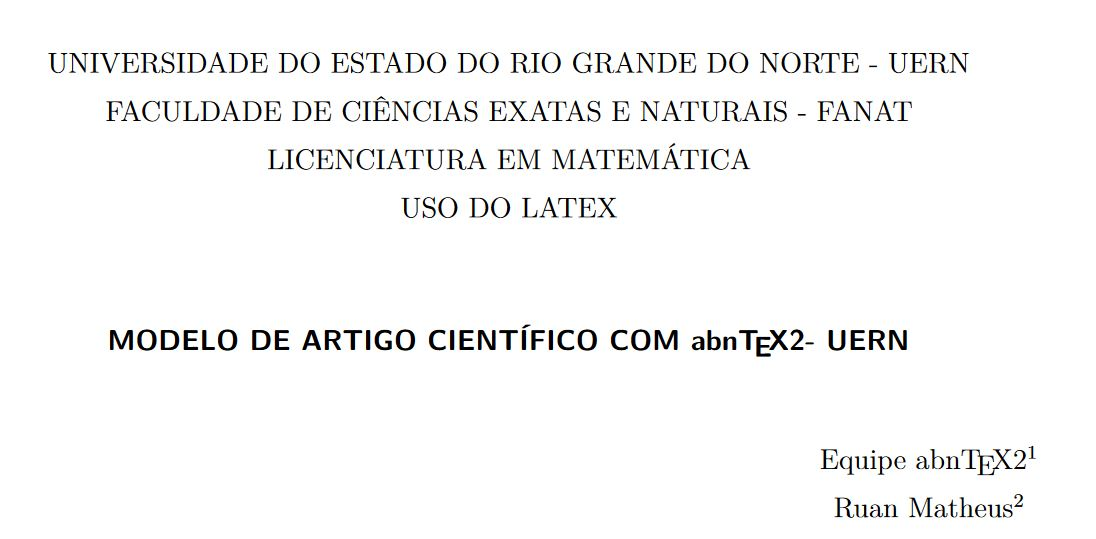
\includegraphics[scale=0.5]{Imagem 1.jpg}
        \caption{Capa com informações complementares}
        \label{fig:enter-label}
    \end{figure}

    \section{PORQUÊ USAR LATEX}

    O editor de texto ideal é aquele que consegue atender às suas necessidades. O \LaTeX $~$ oferece grandes vantagens para quem deseja escrever na área das ciências exatas, pois possibilita a inserção de fórmulas, equações e outros elementos da matemática, física e química de maneira fácil e elegante. Além disso, a classe \abnTeX $~$ oferece toda a formatação exigida pela ABNT de forma simples.

    \subsection{Citações}

    Com a classe \abnTeX $~$, citações com mais de 3 linhas podem ser feitas rapidamente usando o seguinte código:

    \begin{verbatim}
    \begin{citacao}
        Texto da citação [. . .]
    \end{citacao}   
    \end{verbatim}

    Que retornará a seguinte citação:

    \begin{citacao}
        As citações acima de três linhas são conceituadas como longas, não sendo necessário o uso das aspas duplas. No entanto, é obrigatório recuar o texto em 4cm, justificar, diminuir a fonte (tamanho 10), e utilizar o espaçamento 1,0 cm entre linhas. Além disso, as citações com mais de três linhas deverão ser separadas do texto que as precede e as sucede apenas por um espaço simples em branco (MANUAL DE NORMALIZAÇÂO, p. 63).
    \end{citacao}

    \subsection{Fórmulas}

\begin{equation}
    \int_{a}^{b} f(x) \, dx, \quad (a+b)^n= \sum\limits_{k=0}^n \binom{n}{k} a^{n-k} b^{k}, \quad f'(x)= \lim\limits_{h \to 0} \dfrac{f(x+h)- f(x)}{h}
\end{equation} \\\\

    \begin{equation}
    \left[
    \begin{array}{cccc}

        a_{11}  & a_{12} & \cdots & a_{1n}  \\
        a_{2_1} & a_{22} & \cdots & a_{2n} \\ 
        \vdots & \vdots & \vdots ~ \ddots & \vdots \\
        a_{n1} & a_{n2} & \cdots & a_{nn}
    \end{array}
    \right]
    \end{equation} \\\\
    
    \begin{equation}
        ax^2+bx+c=0 \implies x= \begin{dcases*}
        x_1: \dfrac{-b + \sqrt{b^2-4ac} }{2a} \\\\ 
        x_2: \dfrac{-b- \sqrt{b^2-4ac}}{2a}
        \end{dcases*}
    \end{equation} \\\\

    \ch{Na2SO4 ->[ H2O ] Na+ + SO4^2-}

    \ch{( 2 Na+ ,SO4^2- ) + (Ba^2+ , 2 Cl- ) -> BaSO4 v + 2 NaCl}

    \section{CONSIDERAÇÕES FINAIS}

    Em um artigo científico, devemos incluir as referências bibliográficas seguindo as normas definidas pela ABNT. A classe \abnTeX, por padrão, usa o seguinte ambiente para a bibliografia: 
    
      \begin{verbatim}
          \bibliography{arquivo-de-referencias-bib}
      \end{verbatim}  
    onde os itens da referencias bibliográfica são descritos em um arquivo \texttt{.bib} dentro do documento \LaTeX. Isso requer criar uma bibliografia usando o \texttt{bibTex}. Nesse arquivo, optei por usar o ambiente \verb|\begin{thebibliography}| que é mais intuitivo e simples de editar, principalmente se você for novo no \LaTeX. Para criar sua bibliografia, basta apenas editar ou sobrescrever a seção a seguir.

    Esse arquivo foi criado com o intuito de tornar acessível a produção de artigos técnicos/científicos usando o \LaTeX tendo em vista as noras da Universidade Estadual do Rio Grande do Norte - UERN. Sinta-se livre para editar e redistribuir este arquivo. Obrigado! \\\\

    


\renewcommand{\bibname}{\normalsize \bfseries \sffamily REFERÊNCIAS}
\begin{thebibliography}{80}
   \bibitem{Manual técnico} ARAÚJO, Aline Karolina da Silva et al. \textbf{Manual de Normalização de Trabalhos acadêmicos da UERN}. 3. ed. revista e atualizada. Mossoró: Edições UERN, 2022. Disponível em: \url{https://www.uern.br/controledepaginas/manualtcc/arquivos/6762manual_de_tcc_uern_2022_finalizado.pdf}.

   \bibitem{Modelo} ARAUJO, L. C. \textbf{Modelo Canônico de Relatório Técnico e/ou Científico com
abnTeX2}. [S.l.],
2015. Disponível em: \url{http://www.abntex.net.br/}.

\bibitem{Modelo2} ARAUJO, L. C. \textbf{Modelo Canônico de Artigo científico com abnTeX2}. [S.l.], 2015.
Disponível em: \url{http://www.abntex.net.br/}.

\bibitem{ABNT} ASSOCIAÇÃO BRASILEIRA DE NORMAS TÉCNICAS. \textbf{ABNT NBR
14724:2011: Informação e documentação — trabalhos acadêmicos — apresentação}.
Rio de Janeiro, 2011. 15 p.
\end{thebibliography}

\end{document}
